\documentclass[12pt, a4paper, oneside]{ctexart}
\usepackage{amsmath, amsthm, amssymb, bm, color, graphicx, geometry, hyperref, mathrsfs,extarrows, braket}

\linespread{1.5}
%\geometry{left=2.54cm,right=2.54cm,top=3.18cm,bottom=3.18cm}
\geometry{left=1.84cm,right=1.84cm,top=2.18cm,bottom=2.18cm}
\newenvironment{problem}{\par\noindent\textbf{题目. }}{\bigskip\par}
\newenvironment{solution}{\par\noindent\textbf{解答. }}{\bigskip\par}
\newenvironment{note}{\par\noindent\textbf{注记. }}{\bigskip\par}

% 基本信息
\newcommand{\dt}{\today}
\newcommand{\sj}{概率论}
\newcommand{\vt}{吴天阳 2204210460}

\begin{document}

%\pagestyle{empty}
\pagestyle{plain}
\vspace*{-15ex}
\centerline{\begin{tabular}{*3{c}}
    \parbox[t]{0.3\linewidth}{\begin{center}\textbf{日期}\\ \large \textcolor{blue}{\dt}\end{center}} 
    & \parbox[t]{0.3\linewidth}{\begin{center}\textbf{科目}\\ \large \textcolor{blue}{\sj}\end{center}}
    & \parbox[t]{0.3\linewidth}{\begin{center}\textbf{姓名,学号}\\ \large \textcolor{blue}{\vt}\end{center}} \\ \hline
\end{tabular}}
\vspace*{4ex}

\paragraph{习题2.1}
\paragraph{3.}证明:对任意$n$个事件$A_1,\cdots,A_n$,都有
\begin{equation*}
    \textbf{P}\left(\bigcap_{k=1}^nA_k\right)\geqslant\sum_{k=1}^n\textbf{P}(A_k)-n+1
\end{equation*}
\begin{proof}
    利用数学归纳法,当$n=2$时,令$A_1 = A, A_2 = B$,则$A\cup B$可分解为三个集合的不交并,即$A\cup B = AB\cup AB^c\cup A^cB$,由测度的有限可加性,知
    \begin{equation*}
        \begin{aligned}
            \textbf{P}(A\cup B) =&\ \textbf{P}(AB)+\textbf{P}(AB^c)+\textbf{P}(A^cB)\\
            =&\ (\textbf{P}(AB)+\textbf{P}(AB^c))+(\textbf{P}(A^cB)+\textbf{P}(AB))-\textbf{P}(AB)\\
            =&\ \textbf{P}(A)+\textbf{P}(B)-\textbf{P}(AB)
        \end{aligned}
    \end{equation*}

    所以有$\textbf{P}(AB) = \textbf{P}(A)+\textbf{P}(B)-\textbf{P}(A\cup B)$,由于$\textbf{P}(A\cup B)\leqslant 1$,则有
    \begin{equation*}
        \textbf{P}(AB) \geqslant \textbf{P}(A)+\textbf{P}(B)-1
    \end{equation*}

    故$n=2$时,该命题成立。假设该命题在$n$时成立,下面讨论$n+1$的情况,令$\bigcap\limits_{k=1}^nA_k = A$,$A_{n+1} = B$,则由$n=2$时的不等式,知
    \begin{equation*}
        \begin{aligned}
            \textbf{P}(\bigcap_{k=1}^{n+1}A_k)\geqslant&\ \textbf{P}(\bigcap_{k=1}^nA_k)+\textbf{P}(A_{n+1}) - 1\\
            \geqslant & \sum_{k=1}^n\textbf{P}(A_k) - n+1+\textbf{P}(A_{n+1})-1\\
            \geqslant & \sum_{k=1}^{n+1}\textbf{P}(A_k)-n
        \end{aligned}
    \end{equation*}

    故该命题在$n+1$时成立。由数学归纳法知,该命题对于任意的$n\in \mathbb{N}$成立。
\end{proof}
\paragraph{6.}证明:$\textbf{P}(A\triangle B) = \textbf{P}(A)+\textbf{P}(B)-2\textbf{P}(AB)$。
\begin{proof} $A^cB, AB^c, AB$两两不相交,由测度的有限可加性,知
    \begin{equation*}
        \begin{aligned}
            \textbf{P}(A\triangle B) =&\ \textbf{P}(AB^c\cup A^cB)\\
            =&\ \textbf{P}(AB^c)+\textbf{P}(A^cB)\\
            =&\ (\textbf{P}(AB^c)+\textbf{P}(AB))+(\textbf{P}(A^cB)+\textbf{P}(AB))-2\textbf{P}(AB)\\
            =&\ \textbf{P}(A)+\textbf{P}(B)-2\textbf{P}(AB)
        \end{aligned}
    \end{equation*}
\end{proof}

\paragraph{11.}设$\mathscr{O}$为$\mathbb{R}$上的开集的全体,$\mathscr{J}$为其上有理顶点开区间全体。证明:$\mathbb{R}$中的$\text{Borel}$域$\mathscr{B} = \sigma(\mathscr{O}) = \sigma(\mathscr{J})$。
\begin{proof}
    设$\mathscr{A}_1 = \{(a, b):-\infty < a < b < +\infty\},\mathscr{A}_2 = \{\mathbb{R}\text{中全体开集和闭集}\}$,则$\mathscr{A}_1\subset \mathscr{O}\subset \mathscr{A}_2$,由\textbf{定理2.1.2}知,
    \begin{equation*}
        \begin{aligned}
            &\mathscr{B} = \sigma(\mathscr{A}_1)\subset \sigma(\mathscr{O})\subset \sigma(\mathscr{A}_2)=\mathscr{B}\\
            \Rightarrow&\ \sigma(\mathscr{O}) = \mathscr{B}
        \end{aligned}
    \end{equation*}

    由于无理点可以由有理顶点组成的开区间逼近,所以$\sigma(\mathscr{J}) = \sigma(\mathscr{O}) = \mathscr{B}$。
\end{proof}
\paragraph{12.}证明:事件$\sigma$域中的事件数目,如果不是有限个,就一定有不可列无限多个。
\begin{proof}
    
假设$\sigma$域$\mathscr{F}$中的事件数目为可列无限个,记$\mathscr{F}$的基数为$\overline{\overline{\mathscr{F}}}$,则$\overline{\overline{\mathscr{F}}}=\aleph_0$(阿列夫零),由于$\mathscr{F}$所包含的集合个数是无限多个,则一定可以取出两两不相交的集合
\begin{equation*}
    \{A_1,A_2,\cdots, A_n,\cdots\}\subset \mathscr{F}
\end{equation*}

记$B = \{A_1,A_2,\cdots,A_n,\cdots\}$,由$\sigma$域的性质知,$B$的所有子集组成的集合$2^B\subset \mathscr{F}$,则$2^{\aleph_0}\leqslant \overline{\overline{F}} = \aleph_0$,与$2^{\aleph_0} > \aleph_0$矛盾。

故不存在可列无限个事件数目的$\sigma$域。
\end{proof}
\paragraph{习题2.2}
\paragraph{2.}提纲中有$25$个问题,某大学生掌握了其中的$20$个问题。试求:所考的$3$个问题恰好都是该大学生已掌握了的问题的概率。
\begin{solution}
    设$\Omega$为所有可能考的$3$个问题,$A$为考大学生掌握的$3$个问题,则
    \begin{equation*}
        \begin{aligned}
            &|\Omega| = \binom{25}{3}, |A| = \binom{20}{3}\\
            &\textbf{P}(A) = \frac{\binom{20}{3}}{\binom{25}{3}} = \frac{57}{115}
        \end{aligned}
    \end{equation*}
\end{solution}
\paragraph{5.}从装有红、白、黑球各一个的袋中任意有放回地取球,直至$3$种颜色的球都取出过为止。试求取球次数(1)大于$k$;(2)恰为$k$的概率。
\begin{solution}
    (1). 设事件$E_k$为取球的次数大于$k$次,$A_1$为前$k$次取球都没有取过红球,$A_2$为前$k$次取球都没有取过白球,$A_3$为前$k$次取球都没有取过黑球,则$E_k = A_1\cup A_2\cup A_3$,由加法定理知,
    \begin{equation*}
        \textbf{P}(E_k) = \sum_{i=1}^3\textbf{P}(A_i)-\sum_{1\leqslant i < j \leqslant 3}\textbf{P}(A_iA_j) + \textbf{P}(A_1A_2A_3)
    \end{equation*}

    由于三种球的对称性知,
    \begin{equation*}
        \textbf{P}(A_i) = \frac{2^{k}}{3^{k}},\quad \textbf{P}(A_iA_j)=\frac{1}{3^{k}},\quad \textbf{P}(A_1A_2A_3) = 0
    \end{equation*}

    则,
    \begin{equation*}
        \begin{aligned}
            \textbf{P}(E_k) =& \binom{3}{1}\frac{2^{k}}{3^{k}}-\binom{3}{2}\frac{1}{3^{k}}+0\\
            =&\ \frac{2^{k}-1}{3^{k-1}}
        \end{aligned}
    \end{equation*}

    (2). 设事件$B_k$为取球次数恰好为$k$次,则
    \begin{equation*}
        \begin{aligned}
            \textbf{P}(B_k) =&\ \textbf{P}(E_{k-1})-\textbf{P}(E_k)\\
            =&\ \frac{2^{k-1}-1}{3^{k-2}}-\frac{2^{k}-1}{3^{k-1}}\\
            =&\ \frac{2^{k-1}-2}{3^{k-1}}
        \end{aligned}
    \end{equation*}
\end{solution}
\paragraph{7.}向画满间隔为$a$的平行直线的桌面上任意投放一个三角形。假定三角形的三条边长$l_1,l_2,l_3$均小于$a$。求此三角形与某直线相交的概率。
\begin{solution}取该三角形的外接圆,设$E_t$为三角形内部,$E_B$为外接圆的内部,$E_1,E_2,E_3$分别为三个半圆部分,如下图所示

    \centerline{
        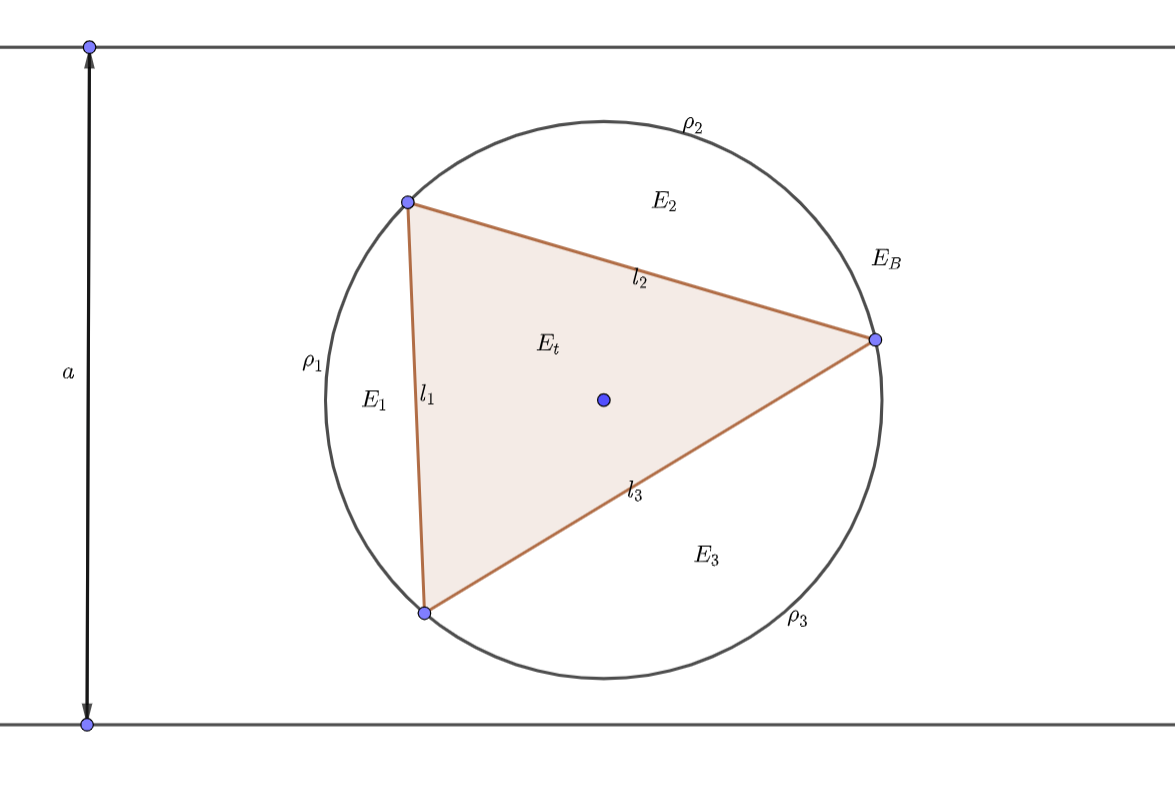
\includegraphics[width=0.8\textwidth]{figure.png}
    }

    则,$E_B=E_t\cup E_1\cup E_2\cup E_3$,由加法定理知,
    \begin{equation*}
        \begin{aligned}
            \textbf{P}(E_B) =&\ \textbf{P}(E_t\cup E_1\cup E_2\cup E_3)\\
            =&\quad\ \,\textbf{P}(E_t)+\textbf{P}(E_1)+\textbf{P}(E_2)+\textbf{P}(E_3)\\
            &\ -\textbf{P}(E_tE_1)-\textbf{P}(E_tE_2)-\textbf{P}(E_tE_3)-\textbf{P}(E_1E_2)-\textbf{P}(E_1E_3)-\textbf{P}(E_2E_3)\\
            &\ +\textbf{P}(E_tE_1E_2)+\textbf{P}(E_tE_2E_3)+\textbf{P}(E_tE_1E_3)+\textbf{P}(E_1E_2E_3)\\
            &\ -\textbf{P}(E_tE_1E_2E_3)
        \end{aligned}
    \end{equation*}

    由之前抛针问题及其推论知,
    \begin{equation*}
        \begin{aligned}
            &\textbf{P}(E_B) = \frac{\rho_1+\rho_2+\rho_3}{\pi a},\quad\textbf{P}(E_i) = \frac{\rho_1+l_1}{\pi a},\quad \textbf{P}(E_tE_i) = \frac{2l_i}{\pi a}\\
            &\textbf{P}(E_iE_j)=\textbf{P}(E_tE_iE_j),\quad \textbf{P}(E_1E_2E_3) = \textbf{P}(E_tE_1E_2E_3)
        \end{aligned}
    \end{equation*}

    则,
    \begin{equation*}
        \begin{aligned}
            \frac{\rho_1+\rho_2+\rho_3}{\pi a} =&\ \textbf{P}(E_t)+\frac{\rho_1+\rho_2+\rho_3+l_1+l_2+l_3-2l_1-2l_2-2l_3}{\pi a}\\
            =&\ \textbf{P}(E_t)+\frac{\rho_1+\rho_2+\rho_3-l_1-l_2-l_3}{\pi a}
        \end{aligned}
    \end{equation*}

    故,
    \begin{equation*}
        \textbf{P}(E_t) = \frac{l_1+l_2+l_3}{\pi a}
    \end{equation*}
\end{solution}
\paragraph{习题2.3}
\paragraph{5.}一学生接连参加同一课程的两次考试,第一次及格的概率为$p$,若第一次及格则第二次及格的概率也为$p$;若第一次不及格则第二次及格的概率为$\frac{p}{2}$。

(1) 若至少有一次及格则他能取得某种资格,求他取得资格的概率。

(2) 若已知第二次及格,求他第一次及格的概率。

\begin{solution}
    设$A$为他第一次及格的事件,$B$为他第二次及格的事件。

    (1) 设$E_1$为至少有一次及格的事件,则$E_1^c$为他全部不及格的事件,
    \begin{equation*}
        \textbf{P}(E_1) = 1-\textbf{P}(E_1^c) = 1-\textbf{P}(A^cB^c) = 1-(1-p)(1-\frac{p}{2}) = \frac{3}{2}p-\frac{p^2}{2}
    \end{equation*}

    (2) 设$E_2$为第二次及格条件下,第一次及格的事件,则$\textbf{P}(E_2) = \textbf{P}(A|B)$,由$\text{Bayes公式}$知,
    \begin{equation*}
        \begin{aligned}
            \textbf{P}(E_2) = \textbf{P}(A|B) =&\ \frac{\textbf{P}(A)\textbf{P}(B|A)}{\textbf{P}(A)\textbf{P}(B|A)+\textbf{P}(A^c)\textbf{P}(B|A^c)}\\
            =&\ \frac{p\cdot p}{p\cdot p+(1-p)\dfrac{p}{2}}\\
            =&\ \frac{2p}{1+p}
        \end{aligned}
    \end{equation*}
\end{solution}
\paragraph{8.}袋中有$2n-1$个白球和$2n$个黑球,现任意取出$n$个,发现它们是同色的,求同为黑色的概率。
\begin{solution}
    设$\Omega$为任取$n$个球的事件,$A$为取$n$个相同颜色球的事件,$B_1$为取$n$个黑球的事件,$B_2$为取$n$个白球的事件。则$B_1\cup B_2 = A, |\Omega| = \binom{4n-1}{n}, |B_1| = \binom{2n}{n}, |B_2| = \binom{2n-1}{n}$

    \begin{equation*}
        \textbf{P}(A) = \textbf{P}(B_1)+\textbf{P}(B_2) = \frac{\binom{2n-1}{n}+\binom{2n}{n}}{\binom{4n-1}{n}}
    \end{equation*}

    所以,

    \begin{equation*}
        \begin{aligned}
            \textbf{P}(B_1|A) = \frac{\textbf{P}(AB_1)}{\textbf{P}(A)} = &\ \frac{\textbf{P}(B_1)}{\textbf{P}(A)}\\
            =&\ \frac{\binom{2n}{n}}{\binom{2n-1}{n}+\binom{2n}{n}}\\
            =&\ \frac{(2n)!}{n(2n-1)!+(2n)!}
        \end{aligned}
    \end{equation*}
\end{solution}
\paragraph{14.}袋中有$r$个红球与$b$个黑球,现任取一球,添加$s$个同色的球一并放回。再从袋中任取出一球发现是红球,求第一次取出的球是黑球的概率。
\begin{solution}
    设$E$为题目问题,$A$为第一次取出的球是黑球的事件,$B$为第二次取出的球是红球的事件,由$\text{Bayes公式}$知,
    \begin{equation*}
        \begin{aligned}
            \textbf{P}(E) = \textbf{P}(A|B) =&\ \frac{\textbf{P}(A)\textbf{P}(B|A)}{\textbf{P}(A)\textbf{P}(B|A)+\textbf{P}(A^c)\textbf{P}(B|A^c)}\\
            =&\ \frac{\frac{b}{r+b}\cdot \frac{r}{r+b+s}}{\frac{b}{r+b}\cdot\frac{r}{r+b+s}+\frac{r}{r+b}\cdot\frac{r+s}{r+b+s}}\\
            =&\ \frac{br}{br+r(r+s)}\\
            =&\ \frac{b}{r+b+s}
        \end{aligned}
    \end{equation*}
\end{solution}
\paragraph{习题2.4}
\paragraph{3.}掷一枚不均匀的硬币$n$次,第$1$次抛出正面的概率为$c$,此后每次掷出与前次相同结果的概率为$p\ (0\leqslant p\leqslant 1)$。求第$n$次抛出正面的概率,并讨论$n\rightarrow \infty$时的极限。
\begin{solution}
    设$A_n$为第$n$次抛出正面的事件,记$p_n = \textbf{P}(A_n)$,由全概率公式知
    \begin{equation*}
        p_n = \textbf{P}(A_n) = \textbf{P}(A_{n-1})\textbf{P}(A_n|A_{n-1})+\textbf{P}(A_{n-1}^c)\textbf{P}(A_n|A_{n-1}^c)
    \end{equation*}
    则
    \begin{equation*}
        \begin{aligned}
            &\ p_n = p_{n-1}\cdot p+(1-p_{n-1})(1-p) = (2p-1)p_{n-1}+1-p\\
            \Rightarrow&\ p_n-\frac{1}{2} = (2p-1)(p_{n-1}-\frac{1}{2})
        \end{aligned}
    \end{equation*}

    且$p_1 = c$,由等比数列通项公式知,
    \begin{equation*}
        \begin{aligned}
            &\ p_n-\frac{1}{2}=(2p-1)^{n-1}(c-\frac{1}{2})\\
            \Rightarrow &\ p_n=\frac{1}{2}+(2p-1)^{n-1}(c-\frac{1}{2})
        \end{aligned}
    \end{equation*}

    当$0<p<1$时,$|2p-1| < 1$,则$(2p-1)^{n-1}\rightarrow 0$,故$\lim\limits_{n\rightarrow \infty}p_n=\dfrac{1}{2}$;

    当$p=1$时,$p_n = c$;

    当$p=0$时,$p_n = \dfrac{1}{2} + (-1)^{n-1}(c-\dfrac{1}{2})$,发散。

    综上,

    \begin{equation*}
        \lim_{n\rightarrow 0}p_n = \begin{cases}
            \text{发散}, &\quad p=0,\\
            \dfrac{1}{2}, &\quad 0<p<1\\
            c, &\quad p=1.
        \end{cases}
    \end{equation*}
\end{solution}
\paragraph{10.}$30$个学生参加考试,其中有$5$个学生一贯优秀,有$10$个学生成绩较好,有$15$个学生学业较差。成绩一贯优秀的学生考试中总得“优秀”;成绩较好的学生以相等的概率考得“优秀”和“良好”;学业成绩较差的学生则以相等的概率考得“良好”,“及格”和“不及格”。随机叫出一个学生,试求他的考试结果为:(1) “优秀”;(2) “良好”的概率。
\begin{solution}
    设$A_1,A_2$分别表示叫出的学生考试成绩为“优秀”,“良好”的事件,$B_1,B_2,B_3$分别表示叫出一贯优秀,成绩较好,成绩较差的学生的事件,由全概率公式知,
    \begin{equation*}
        \begin{aligned}
            \textbf{P}(A_1) =&\ \textbf{P}(B_1)\textbf{P}(A_1|B_1)+\textbf{P}(B_2)\textbf{P}(A_1|B_2)+\textbf{P}(B_3)\textbf{P}(A_1|B_3)\\
            =&\ \frac{5}{30}\cdot 1+\frac{10}{30}\cdot \frac{1}{2}+\frac{15}{30}\cdot 0\\
            =&\ \frac{1}{3}
        \end{aligned}
    \end{equation*}
    \begin{equation*}
        \begin{aligned}
            \textbf{P}(A_2) =&\ \textbf{P}(B_1)\textbf{P}(A_2|B_1)+\textbf{P}(B_2)\textbf{P}(A_2|B_2)+\textbf{P}(B_3)\textbf{P}(A_2|B_3)\\
            =&\ \frac{5}{30}\cdot 0+\frac{10}{30}\cdot \frac{1}{2}+\frac{15}{30}\cdot \frac{1}{3}\\
            =&\ \frac{1}{3}
        \end{aligned}
    \end{equation*}
\end{solution}
\paragraph{17.}(选票问题)在一次选举中,候选人$A$得到$n$张选票而候选人$B$得到$m$张选票,其中$n>m$,假定选票的一切排列次序是等可能的,证明:在计票过程中,$A$的票数始终领先的概率为$\dfrac{n-m}{n+m}$。
\begin{proof}
    设$E$为候选人$A$的选票一直领先候选人$B$的选票的事件,$H$为在计票过程中出现了候选人$B$的票数多于候选人$A$的事件,事件$H$又可以分为两类,第一次计票结果为候选人$B$,记为$H_1$,第一次计票结果为候选人$A$,则为$H_1^c$,由反射原理知,$|H_1| = |H_1^c|$,则只需考虑$H_1$中的样本个数。

    由于最终一定是候选人$A$的票数多于候选人$B$的票数,所以只需考虑剩余选票的排列即可,则
    \begin{equation*}
        |H_1| = \binom{n+m-1}{n}
    \end{equation*}

    设样本空间$|\Omega|$为所有的选票排列集合,则$|\Omega| = \binom{n+m}{n}$,又由于$E$与$H$为对立事件,所以
    \begin{equation*}
        \begin{aligned}
            \textbf{P}(E) =&\ 1-\textbf{P}(H)=1-\frac{|H|}{|\Omega|}= 1-\frac{2|H_1|}{|\Omega|}\\
            =&\ 1-\frac{2\binom{n+m-1}{n}}{\binom{n+m}{n}} =\ 1-\frac{2\frac{(n+m-1)!}{n!(m-1)!}}{\frac{(n+m)!}{n!m!}}   = 1-\frac{2m}{n+m}\\
            =&\ \frac{n-m}{n+m}
        \end{aligned}
    \end{equation*}
\end{proof}
\paragraph{习题2.5}
\paragraph{3.}无线电监测站负责监测$n$个目标。假定在监测过程中第$i$个目标消失的概率为$p_i$,且各目标是否消失相互独立。求下列事件的概率:(1) 监测过程中没有目标消失;(2) 至少一个目标消失;(3) 不多于一个目标消失。

\begin{solution}
    设$E_1,E_2,E_3$分别表示题目所问的三个事件,$A_i$表示第$i$个目标消失的事件,则$A_i$和$A_i^c\ (i=1,2,\cdots, n)$均两两独立。
    \begin{equation*}
        \textbf{P}(E_1) = \textbf{P}\left(\bigcap_{i=1}^nA_i^c\right) = \prod_{i=1}^n\textbf{P}(A_i^c) = \prod_{i=1}^n(1-p_i)
    \end{equation*}

    \begin{equation*}
        \textbf{P}(E_2) = 1-\textbf{P}(E_1) = 1-\prod_{i=1}^n(1-p_i)
    \end{equation*}

    设$B$表示只有一个目标消失的事件,$B_i$表示只有第$i$个目标消失的事件,则
    \begin{equation*}
        \textbf{P}(B_i) = \textbf{P}(A_1^cA_2^c\cdots A_i\cdots A_n^c) = p(1-p)^{n-1}
    \end{equation*}
    \begin{equation*}
        \textbf{P}(B) = \textbf{P}\left(\bigcup_{i=1}^nB_i\right) = \sum_{i=1}^n\textbf{P}(B_i) = np(1-p)^{n-1}
    \end{equation*}
    \begin{equation*}
        \textbf{P}(E_3) = \textbf{P}(E_1) + \textbf{P}(B) = \prod_{i=1}^n(1-p_i) + np(1-p)^{n-1}
    \end{equation*}
\end{solution}
\paragraph{4.}当开关$K_1$断开,或开关$K_2$与$K_3$同时断开时电路断开。设$K_1,K_2,K_3$断开的概率依次是$0.4,0.5,0.7$,且各开关相互独立。求电路断开的概率。
\begin{solution}
    设$E$为电路断开的事件,$A_i$为开关$K_i$断开的事件$(i=1,2,3)$,由题意可知
    \begin{equation*}
        \begin{aligned}
            \textbf{P}(E) =&\ \textbf{P}(A_1\cup(A_2A_3))\\
            =&\ 1-(1-\textbf{P}(A_1))(1-\textbf{P}(A_2A_3))\\
            =&\ 1-(1-0.4)(1-0.5\cdot 0.7)\\
            =&\ 0.61
        \end{aligned}
    \end{equation*}
\end{solution}
\paragraph{8.}考察正方体各个面的中心。甲、乙二人相互独立地从中分别选取$3$个点连成三角形,试求所得的两个三角形彼此全等的概率。
\begin{solution}
    设$E$为两个三角形彼此全等的事件,$A_1,A_2$分别为甲、乙选到等边三角形的事件。由于正方形一共有$6$个面的中心,则总的三角形选择方法一共有$|\Omega| = \binom{6}{3} = 20$种,且选出的三角形要么是等边三角形要么是直角三角形,且等边三角形的个数等于正方形顶角的个数,即$8$个,所以
    \begin{equation*}
        \textbf{P}(A_1) = \textbf{P}(A_2) = \frac{8}{20} = \frac{2}{5}
    \end{equation*}

    则

    \begin{equation*}
        \begin{aligned}
            \textbf{P}(E) =&\ \textbf{P}(A_1A_2\cup A_1^cA_2^c) = \textbf{P}(A_1A_2)+\textbf{P}(A_1^cA_2^c)\\
            =&\ \textbf{P}(A_1)\textbf{P}(A_2) + \textbf{P}(A_1^c)\textbf{P}(A_2^c)=\frac{2}{5}\cdot \frac{2}{5} + \frac{3}{5} \cdot \frac{3}{5}\\
            =&\ \frac{13}{25}
        \end{aligned}
    \end{equation*}
\end{solution}
\paragraph{12.}在$18$次独立重复的$\text{Bernoulli}$试验中,事件$A$发生的概率都等于$0.2$,求该事件至少发生$3$次的概率。
\begin{solution}
    设$E$为题目所问的事件,$E_i$表示事件发生$i$次的概率,$A_i$为事件$A$在第$i$次重复试验中发生的事件,则
    \begin{equation*}
        \begin{aligned}
            &\textbf{P}(E_0) = \textbf{P}\left(\bigcap_{i=1}^{18}A_i^c\right) = 0.8^{18}\\
            &\textbf{P}(E_1) = \textbf{P}\left(\bigcup_{i=1}^{18}A_1^c\cdots A_{i-1}^cA_iA_{i+1}^c\cdots A_n^c\right) = 18\cdot 0.2\cdot 0.8^{17}\\
            &\textbf{P}(E_2) = \textbf{P}\left(\bigcup_{1\leqslant i < j\leqslant 18}A_1^c\cdots A_{i-1}^cA_iA_{i+1}^c\cdots A_{j-1}^cA_jA_{j+1}^c\cdots A_{n}^c\right) = \binom{18}{2}0.2^2\cdot 0.8^{16}
        \end{aligned}
    \end{equation*}

    所以
    \begin{equation*}
        \textbf{P}(E) = 1-\textbf{P}(E_0\cup E_1\cup E_2) = 1-0.8^{18}-18\cdot 0.2\cdot 0.8^{17}-\binom{18}{2} 0.2^2\cdot 0.8^{16} \thickapprox 0.728658
    \end{equation*}
\end{solution}
\paragraph{18.}证明:如果$\textbf{P}(A|B)=\textbf{P}(A|B^c)$,则事件$A$与$B$独立。
\begin{proof}
    由于$\textbf{P}(A) = \textbf{P}(AB)+\textbf{P}(AB^c)$,则
    \begin{equation*}
        \begin{aligned}
            &\ \textbf{P}(A|B^c) = \frac{\textbf{P}(AB^c)}{\textbf{P}(B^c)}=\frac{\textbf{P}(A)-\textbf{P}(AB)}{1-\textbf{P}(B)}=\textbf{P}(A|B) = \frac{\textbf{P}(AB)}{\textbf{P}(B)}\\
            \Rightarrow&\ \textbf{P}(B)(\textbf{P}(A)-\textbf{P}(AB)) = \textbf{P}(AB)-\textbf{P}(B)\textbf{P}(AB)\\
            \Rightarrow&\ \textbf{P}(AB) = \textbf{P}(A)\textbf{P}(B)
        \end{aligned}
    \end{equation*}

    综上,事件$A$与$B$独立。
\end{proof}
\end{document}
